\documentclass[a4paper,12pt]{article}
\usepackage{fullpage}
\usepackage[british]{babel}

\usepackage{amsmath}
\usepackage{amssymb}
\usepackage{amsthm} \newtheorem{theorem}{Theorem}
\usepackage{color}
\usepackage{float}
\usepackage{listings}
\usepackage{subfig}
\lstset{% parameters for all code listings
	language=Python,
	frame=single,
	basicstyle=\small,  % nothing smaller than \footnotesize, please
	tabsize=2,
	numbers=left,
	framexleftmargin=2em,  % extend frame to include line numbers
	%xrightmargin=2em,  % extra space to fit 79 characters
	breaklines=true,
	breakatwhitespace=true,
	prebreak={/},
	captionpos=b,
	columns=fullflexible,
	escapeinside={\#*}{\^^M}
}
\usepackage{fancyvrb}
\DefineVerbatimEnvironment{code}{Verbatim}{fontsize=\small}
\DefineVerbatimEnvironment{example}{Verbatim}{fontsize=\small}

\usepackage{tikz} \usetikzlibrary{trees}
\usepackage{hyperref}  % should always be the last package

% useful colours (use sparingly!):
\newcommand{\blue}[1]{{\color{blue}#1}}
\newcommand{\green}[1]{{\color{green}#1}}
\newcommand{\red}[1]{{\color{red}#1}}

% useful wrappers for algorithmic/Python notation:
\newcommand{\length}[1]{\text{len}(#1)}
\newcommand{\twodots}{\mathinner{\ldotp\ldotp}}  % taken from clrscode3e.sty
\newcommand{\Oh}[1]{\mathcal{O}\left(#1\right)}

% useful (wrappers for) math symbols:
\newcommand{\Cardinality}[1]{\left\lvert#1\right\rvert}
%\newcommand{\Cardinality}[1]{\##1}
\newcommand{\Ceiling}[1]{\left\lceil#1\right\rceil}
\newcommand{\Floor}[1]{\left\lfloor#1\right\rfloor}
\newcommand{\Iff}{\Leftrightarrow}
\newcommand{\Implies}{\Rightarrow}
\newcommand{\Intersect}{\cap}
\newcommand{\Sequence}[1]{\left[#1\right]}
\newcommand{\Set}[1]{\left\{#1\right\}}
\newcommand{\SetComp}[2]{\Set{#1\SuchThat#2}}
\newcommand{\SuchThat}{\mid}
\newcommand{\Tuple}[1]{\langle#1\rangle}
\newcommand{\Union}{\cup}
\usetikzlibrary{positioning,shapes,shadows,arrows}


\title{\textbf{Evolutionary Simulator In A Dynamic Environment}}

\author{Jonathan Sharyari \and Lukas Klingsbo}  % replace by your name(s)

%\date{Month Day, Year}
\date{\today}

\begin{document}

\maketitle

\section{Abstract}

\section{Introduction}
Genetic algorithms (GAs) are a common tool to find solutions to complex problems, often with high dimensionality. Although much research has been done on the subject, this research has to some extent focused on problems in a stationary environment. Since in a dynamic environment, the fitness function changes over time a traditional GA is not very suited for solving dynamic problems, as it is likely that the population will quickly converge and not be able to adapt when the fitness function changes. [referens?]

Several approaches have been proposed in order to allow GAs to maintain the population diversity, two common methods are \emph{random immigrants} and \emph{triggered hypermutation} [1][2].

\section{Environment}
Our test environment consists of a simple map, containing food, and is randomely initialized. The goal of the population is to find paths leading to areas where food is distributed. A dynamic environment is created by changing the positions of the food in the map. This can be done in many ways, and we settle for three different methods of changing the map.

\begin{itemize}

\item
Evolving map- Small changes are done, but fairly often. The optimum after a change will lie close to the earlier optimum.
\item
Shotgun map - The map is reinitialized, changing the positions of obstacles and enemies. This must be done rarely, as to give the population the time to readapt.
\item
Seasonal map - similar to the shotgun map, changes are large and rare, but the number of maps is finite and periodic.
\end{itemize}

We anticipate that different dynamic methods (see below) will have the best performance on the different types of map.

\section{Suggested Dynamic Methods}
\subsection{Hypermutation}
The concept of mutation is critical for genetic algorithms, as it is through mutation a genetic algorithm maintains its diversity. As the problem of training in a dynamic environment is to avoid or overcome early convergence, it is tempting to try training with a higher degree of mutation than commonly used in static environments. This is a very simple concept, but the results obtained in [1] show that the pef

\subsection{Triggered Hypermutation}
A higher mutation rate results in higher diversity as indicated above, but a high mutation rate makes it difficult to converge. The mutation rate is therefore generally kept low in standard GAs. The method of using a high mutation rate in a dynamic system might therefore lead to non-converging individuals.

Triggered hypermutation is a proposed solution to this problem. The mutation rate in general is kept low, giving better convergence. When the system is altered in a way that decreases the fitness, the hypermutation stage is started and the mutation rate is temporarily increased giving the same effect as the method explained above.

\subsection{Immigrants}
Random immigrants and elitism-based immigrants use a different approach to maintain diversity. In these methods, some individuals with low fitness are removed and replaced with new individuals.

With random immigrants, these new individuals are randomely created (the same way individuals were initialized at the beginning).

With elitism-based immigrants, the individuals with high fitness are remembered. When the total fitness decreases (potentially due to changes in the environment), individuals with low fitness are removed and individuals from this elite-set are reintroduced.

\section{Genome representation}
The behavior of an individual depends on its genome, which decides how it moves on the map. The genome is represented as a matrix of vector values where each position in the matrix represents a part of the map, and the vector stored at the position is the direction in which the individual will move. For a matrix of size $m \times n$, this is represented as m arrays of size n.

Consider a map of size $50m \times 50n$ and a matrix of size $m \times n$. Then every matrix position will represent a $50\times50$ square in the map. When the individual has a position inside that square, it's speed and direction will be given by the vector stored in that position of the matrix.

\section{Selection and Crossover strategies}
Two different crossover types where used, epoch and collision learning. In collision learning, the individuals crossover when they collide in the map, provided they have collected some ammount of food. Two new individuals are created by one either one-point, two-point or uniform crossover.

In epoch learning, the individuals search the map for a fixed set of updates, one epoch. At the end of the epoch, individuals were recombinated and mutated depending on the settings used. The selection method used worked by first sorting the list of individuals, with the highest fitness first, using the number of food collected as a measure of the fitness. Then, each individual from the beginning crosses over with a probability $\alpha$ with the first individual. If not, the individual crosses over with the same probability $\alpha$ with the second individual, and so on. In general, only the best half of the individuals reproduce.


\section{Discussion}
\subsection{genome representation}
The genome is represented as an array of arrays. During a crossover, assume 1-point, the crossover will be row by row until the point of crossover, but could not be column by column. This means the representation will be much more effective if the target (the food) lies in the top of the map than in the bottom. See illustration.

\begin{figure}
  \caption{}
  \centering
    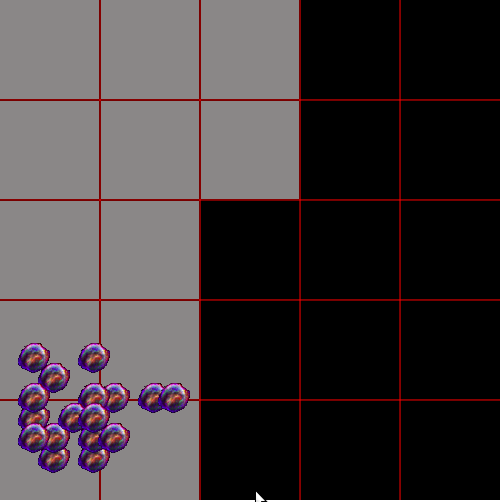
\includegraphics[width=0.5\textwidth]{BottomLeft.png}
    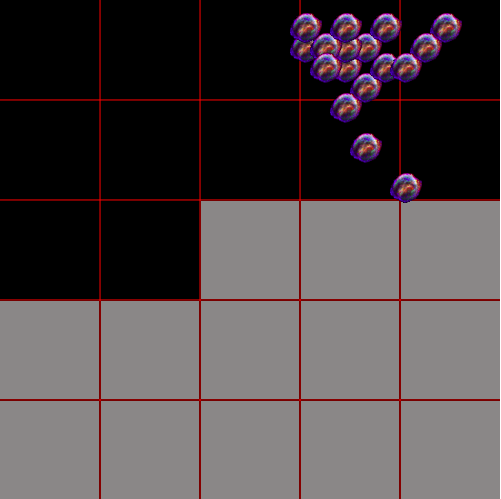
\includegraphics[width=0.5\textwidth]{TopRight.png}
\end{figure}


\section{Conclusions}

\section{references}
[1] H. G. Cobb, J. J. Grefenstette (1993) Genetic Algorithms for Tracking Changing Environments, Proceedings of the 5th International Conference on Genetic Algorithms
[2] A. Simões, E. Costa (2002) Using Genetic Algorithms to Deal with Dynamic Environments: A Comparative Study of Several Approaches Based on Promoting Diversity, GECCO '02 Proceedings of the Genetic and Evolutionary Computation Conference
[3]

\end{document}

